%%%%%%%%%%%%%%%%%%%%%%%%%%%%%%%%%%%%%%%%%%%%%%%%%%%%%%%%%%%%%%%%%%%%%%%%%%%%%%%%
% File acl2014.tex
%
% Contact: koller@ling.uni-potsdam.de, yusuke@nii.ac.jp
%
% Based on the style files for ACL-2013, which were, in turn,
% Based on the style files for ACL-2012, which were, in turn,
% based on the style files for ACL-2011, which were, in turn, 
% based on the style files for ACL-2010, which were, in turn, 
% based on the style files for ACL-IJCNLP-2009, which were, in turn,
% based on the style files for EACL-2009 and IJCNLP-2008...
%
% Based on the style files for EACL 2006 by 
% e.agirre@ehu.es or Sergi.Balari@uab.es
% and that of ACL 08 by Joakim Nivre and Noah Smith

\documentclass[11pt]{article}
\usepackage{acl2014}
\usepackage{times}
\usepackage{url}
\usepackage{latexsym}

%\setlength\titlebox{5cm}

\usepackage[utf8]{inputenc}
\usepackage[usenames,dvipsnames]{xcolor}
\usepackage{tikz}

\usetikzlibrary{shapes}

\newtheorem{definition}{Definition}
\newtheorem{property}{Property}

\newcommand\TODO[1]{\textcolor{red}{[TODO #1]}}

% TikZ database node
% http://tex.stackexchange.com/questions/123854/display-database-instance-relationship-with-tikz
\tikzstyle{database}=[
  draw,
  align=center,
  minimum width=5.5em,
  minimum height=6.5em,
  cylinder,
  cylinder uses custom fill,
  cylinder body fill=white,
  cylinder end fill=white,
  shape border rotate=90,
  aspect=0.5
]

% TikZ document node
% http://tex.stackexchange.com/questions/103688/folded-paper-shape-tikz
\makeatletter
\pgfdeclareshape{doc}{
  \inheritsavedanchors[from=rectangle] % this is nearly a rectangle
  \inheritanchorborder[from=rectangle]
  \inheritanchor[from=rectangle]{center}
  \inheritanchor[from=rectangle]{north}
  \inheritanchor[from=rectangle]{south}
  \inheritanchor[from=rectangle]{west}
  \inheritanchor[from=rectangle]{east}
  % ... and possibly more
  \backgroundpath{% this is new
    % store lower right in xa/ya and upper right in xb/yb
    \southwest \pgf@xa=\pgf@x \pgf@ya=\pgf@y
    \northeast \pgf@xb=\pgf@x \pgf@yb=\pgf@y
    % compute corner of ‘‘flipped page’’
    \pgf@xc=\pgf@xb \advance\pgf@xc by-10pt % this should be a parameter
    \pgf@yc=\pgf@yb \advance\pgf@yc by-10pt
    % construct main path
    \pgfpathmoveto{\pgfpoint{\pgf@xa}{\pgf@ya}}
    \pgfpathlineto{\pgfpoint{\pgf@xa}{\pgf@yb}}
    \pgfpathlineto{\pgfpoint{\pgf@xc}{\pgf@yb}}
    \pgfpathlineto{\pgfpoint{\pgf@xb}{\pgf@yc}}
    \pgfpathlineto{\pgfpoint{\pgf@xb}{\pgf@ya}}
    \pgfpathclose
    % add little corner
    \pgfpathmoveto{\pgfpoint{\pgf@xc}{\pgf@yb}}
    \pgfpathlineto{\pgfpoint{\pgf@xc}{\pgf@yc}}
    \pgfpathlineto{\pgfpoint{\pgf@xb}{\pgf@yc}}
    \pgfpathlineto{\pgfpoint{\pgf@xc}{\pgf@yc}}
  }
}
\makeatother
\tikzstyle{document}=[
  draw,
  align=center,
  color=black,
  fill=white,
  minimum width=5.5em,
  minimum height=6.5em,
  shape=doc,
  inner sep=2ex
]
\newcommand\drawdatabase[1]{
  \begin{tikzpicture}
    \node[database] (database) {#1};
  \end{tikzpicture}
}
\newcommand\drawdocument[1]{
  \begin{tikzpicture}
    \node[document] (document) {#1};
  \end{tikzpicture}
}
\newcommand\drawcorpus[1]{
  \begin{tikzpicture}
    \node[document] (background) {#1};
    \node[document] at ([xshift=.25em, yshift=-.25em]background) (middle) {#1};
    \node[document] at ([xshift=.25em, yshift=-.25em]middle) (foreground) {#1};
  \end{tikzpicture}
}

\title{Association-Based Keyphrase Indexing of Bibliographic Records}

%\author{
%  Adrien Bougouin \and Florian Boudin \and Béatrice Daille\\
%  Université de Nantes, LINA, France\\
%  \normalsize\texttt{\{adrien.bougouin,florian.boudin,beatrice.daille\}@univ-nantes.fr}
%}

\date{}

\begin{document}
  \maketitle
  \begin{abstract}
  \end{abstract}

  \section{Introduction}
\label{sec:introduction}
  % * définition de terme-clé, applications et enjeux
  Un terme-clé est un mot ou une expression polylexicale qui représente un
  concept important d'un document auquel il est associé. En pratique, plusieurs
  termes-clés représentant des concepts différents sont associés à un même
  document. Ils forment alors un ensemble de termes-clés à partir duquel il est
  possible de déduire le contenu principal du document. Du fait de leur capacité
  à synthétiser le contenu d'un document, les termes-clés sont utilisés dans
  diverses applications en Recherche d'Information (RI)~: résumé
  automatique~\cite{avanzo2005keyphrase}, classification de
  documents~\cite{han2007webdocumentclustering}, indexation
  automatique~\cite{medelyan2008smalltrainingset}, etc. Avec l'essor du
  numérique, de plus en plus de documents (articles scientifiques, articles
  journalistiques, etc.) sont accessibles depuis des médiums d'informations tels
  que Internet. Afin de permettre à un utilisateur de rapidement trouver des
  documents, ainsi que d'avoir un bref aperçu de leur contenu, les tâches
  sus-mentionnées sont nécessaires.
  Cependant, la majorité des documents ne sont pas associés avec des termes-clés
  et, compte tenu du nombre important de documents numériques, l'ajout manuel de
  ces derniers n'est pas envisageable. Pour pallier ce problème, de plus en plus
  de chercheurs s'intéressent à l'extraction automatique de termes-clés et
  certaines campagnes d'évaluations, telles que DEFT~\cite{paroubek2012deft} et
  SemEval~\cite{kim2010semeval}, proposent des tâches d'extraction automatique
  de termes-clés.

  % * qu'est-ce que l'extraction automatique de termes-clés
  % * deux écoles : indexation libre et indexation contrôlée (assignation de
  %                 termes-clés)
  %   -> nous sommes de la première école
  % * deux catégories de méthodes : supervisées et non-supervisées
  %    -> en supervisé ils utilisent la structure des documents
  %    -> très peu de travaux en non-supervisé (filtrage des candidats)
  L'extraction automatique de termes-clés, ou indexation libre, est la tâche qui
  consiste à extraire les unités textuelles les plus importantes d'un document,
  en opposition à la tâche d'assignation automatique de termes-clés, ou
  indexation contrôlée, qui consiste à assigner des termes-clés à partir d'une
  terminologie donnée~\cite{paroubek2012deft}. Parmi les méthodes d'extraction
  automatique de termes-clés existantes, nous distinguons deux catégories~: les
  méthodes supervisées et les méthodes non-supervisées. Dans le cas supervisé,
  la tâche d'extraction de termes-clés est considérée comme une tâche de
  classification binaire~\cite{witten1999kea}, où il s'agit d'attribuer la
  classe \og{}\textit{terme-clé}\fg{} ou \og{}\textit{non terme-clé}\fg{} aux
  termes-clés candidats extraits du document. Une collection de documents
  annotés en termes-clés est alors nécessaire pour l'apprentissage d'un modèle
  de classification reposant sur divers traits, allant de la simple fréquence
  aux informations structurelles du document (titre, résumé, introduction,
  conclusion, etc.). Dans le cas non-supervisé, les méthodes attribuent un
  score d'importance à chaque candidat en fonction de divers indicateurs tels
  que la fréquence et la position de la première occurrence dans le document.
  Bien que les méthodes supervisées soient en général plus performantes, la
  faible quantité de documents annotés en termes-clés disponibles, ainsi que la
  forte dépendance des modèles de classification au type des documents à partir
  desquels ils sont appris, poussent les chercheurs à s'intéresser de plus en
  plus aux méthodes non-supervisées.

  % * ici, on cherche à identifier l'échelle de difficulté d'indexation des
  %   documents en Sciences Humaines et Sociales (SHS)
  % * on dispose de 4 collections de notices de 4 disciplines différentes de
  %   SHS + 1 collection de notices de chimie (science dure)
  Dans cette article, nous nous intéressons à l'extraction non-supervisée de
  termes-clés dans les articles scientifiques, et plus particulièrement à la
  performance des méthodes d'extraction de termes-clés dans des domaines de
  spécialité. Au moyen de cinq corpus disciplinaires, notre objectif est
  d'observer et d'analyser l'échelle de difficulté pour l'extraction
  automatique de termes-clés dans des articles scientifiques appartenant à cinq
  disciplines différentes~: Archéologie, Sciences de l'Information,
  Linguistique, Psychologie et Chimie.
  \TODO{Dire pourquoi nous nous intéressons aux méthodes non-supervisées}
  \TODO{Dire pourquoi nous nous intéressons aux articles scientifiques}

  % * annonce du plan
  L'article est structuré comme suit. Un bref état de l'art est donné dans la
  section~\ref{sec:etat_de_l_art}, les données utilisées sont présentées dans la
  section~\ref{sec:presentation_des_donnees} et les expériences menées, ainsi
  que les résultats obtenus, sont décrits dans la section~\ref{sec:experiences}.
  Enfin, une analyse des résultats est donnée dans la
  section~\ref{sec:discussion}, puis une conclusion générale et des perspectives
  de travaux futurs sont présentés en
  section~\ref{sec:conclusion_et_perspectives}.


  %\section{Related Work}
  \begin{frame}{Related Work}
    \framesubtitle{Unsupervised Methods}

    Mostly ranking technics using:
    \begin{itemize}
      \item{language models}
      \item<2->{clusters}
      \item<3->{or \textbf{graphs} of word
                co-occurrences}
      \begin{itemize}
        \item<4->{weighted with co-occurrence number or semantic measure}
        \item<5->{refined with similar documents}
        \item<6->{biased with topic probabilities}
      \end{itemize}
    \end{itemize}
    \vfill
    \alt<6>{
      \cite{liu2010topicalpagerank}
    }{
      \alt<5>{
        \cite{wan2008expandrank}
      }{
        \alt<4>{
          \cite{wan2008expandrank, tsatsaronis2010semanticrank}
        }{
          \alt<3>{
            \cite{mihalcea2004textrank}
          }{
            \alt<2>{
              \cite{liu2009keycluster}
            }{
              \cite{tomokiyo2003languagemodel}
            }
          }
        }
      }
    }
  \end{frame}

  \begin{frame}{Related Work}
    \framesubtitle{Graph-Based Approach: Example (TextRank) and Drawbacks}

    \begin{columns}
      \begin{column}{.6\textwidth}
        \centering
        \alt<3->{
          \begin{tikzpicture}[thin,
                              auto,
                              scale=.25,
                              align=center,
                              node distance=2cm,
                              every node/.style={font=\small, transform shape},
                              main node/.style={text centered,
                                                thick,
                                                fill=JungleGreen!20,
                                                inner sep=1.5pt,
                                                font=\Large\bfseries}]
            % connected component
            \node[main node, fill=BurntOrange!50] (university) {university};
            \node[main node] (duke) [above left=of university.north] {duke};
            \node[main node] (library) [above=of university.north east] {library};
            \node[main node] (press) [below left=of university.south] {press};
            \node[main node] (cornell) [below right=of university.south] {cornell};

            \path[JungleGreen!50] (university) edge (library);
            \path[JungleGreen!50] (university) edge (duke);
            \path[JungleGreen!50] (university) edge (press);
            \path[JungleGreen!50] (university) edge (cornell);

            % connected component
            \node[main node] (further) [left=of university.south west] {further};
            \node[main node] (skills) [below=of further.south west] {skills};

            \path[JungleGreen!50] (skills) edge (further);

            % connected component
            \node[main node, fill=BurntOrange!50] (scholarly) [right=of library.north east] {scholarly};
            \node[main node] (communication) [below=of scholarly.west] {communication};
            \node[main node, fill=BurntOrange!50] (publishing) [below right=of scholarly.south] {publishing};
            \node[main node] (scene) [above right=of publishing.west] {scene};
            \node[main node] (initiative) [below=of publishing.west] {initiative};
            \node[main node, fill=BurntOrange!50] (journal) [below right=of scene.north east] {journal};
            \node[main node, fill=BurntOrange!50] (electronic) [below=of journal.east] {electronic};
            \node[main node] (joint) [below=of electronic.north west] {joint};

            \path[JungleGreen!50] (communication) edge (scholarly);
            \path[JungleGreen!50] (publishing) edge (scholarly);
            \path[JungleGreen!50] (publishing) edge (scene);
            \path[JungleGreen!50] (publishing) edge (journal);
            \path[JungleGreen!50] (publishing) edge (initiative);
            \path[JungleGreen!50] (journal) edge (electronic);
            \path[JungleGreen!50] (joint) edge (electronic);

            % connected component
            \node[main node] (new) [below=of skills.south] {new};
            \node[main node, fill=BurntOrange!50] (role) [below=of new.south east] {role};

            \path[JungleGreen!50] (new) edge (role);

            % connected component
            \node[main node] (digital) [right=of new.south east] {digital};
            \node[main node, fill=BurntOrange!50] (libraries) [below =of cornell.south] {libraries};
            \node[main node] (research) [right =of libraries.south east] {research};

            \path[JungleGreen!50] (digital) edge (libraries);
            \path[JungleGreen!50] (libraries) edge (research);

            % connected component
            \node[main node, fill=BurntOrange!50] (relevant) [below right=of research.north] {relevant};
            \node[main node] (experience) [below left=of relevant.south west] {experience};

            \path[JungleGreen!50] (relevant) edge (experience);

            % connected component
            \node[main node] (model) [below=of digital.south east] {model};
            \node[main node, fill=BurntOrange!50] (economic) [below right=of model.south east] {economic};

            \path[JungleGreen!50] (model) edge (economic);

            % connected component
            \node[main node] (specific) [below left=of economic.center] {specific};
            \node[main node] (aspects) [above left=of specific.north west] {aspects};

            \path[JungleGreen!50] (specific) edge (aspects);

            % connected component
            \node[main node] (life) [below right=of economic.south east] {life};
            \node[main node] (cycle) [right=of life.north east] {cycle};

            \path[JungleGreen!50] (life) edge (cycle);

            % connected component
            \node[main node] (euclid) [right=of relevant.north east] {euclid};
            \node[main node, fill=BurntOrange!50] (project) [below left=of euclid.south east] {project};
            \node[main node] (such) [below left=of project.south east] {such};

            \path[JungleGreen!50] (euclid) edge (project);
            \path[JungleGreen!50] (project) edge (such);
          \end{tikzpicture}
        }{
          \begin{tikzpicture}[thin,
                              auto,
                              scale=.25,
                              align=center,
                              node distance=2cm,
                              every node/.style={font=\small, transform shape},
                              main node/.style={text centered,
                                                thick,
                                                fill=JungleGreen!20,
                                                inner sep=1.5pt,
                                                font=\Large\bfseries}]
            % connected component
            \node[main node] (university) {university};
            \node[main node] (duke) [above left=of university.north] {duke};
            \node[main node] (library) [above=of university.north east] {library};
            \node[main node] (press) [below left=of university.south] {press};
            \node[main node] (cornell) [below right=of university.south] {cornell};

            \path[JungleGreen!50] (university) edge (library);
            \path[JungleGreen!50] (university) edge (duke);
            \path[JungleGreen!50] (university) edge (press);
            \path[JungleGreen!50] (university) edge (cornell);

            % connected component
            \node[main node] (further) [left=of university.south west] {further};
            \node[main node] (skills) [below=of further.south west] {skills};

            \path[JungleGreen!50] (skills) edge (further);

            % connected component
            \node[main node] (scholarly) [right=of library.north east] {scholarly};
            \node[main node] (communication) [below=of scholarly.west] {communication};
            \node[main node] (publishing) [below right=of scholarly.south] {publishing};
            \node[main node] (scene) [above right=of publishing.west] {scene};
            \node[main node] (initiative) [below=of publishing.west] {initiative};
            \node[main node] (journal) [below right=of scene.north east] {journal};
            \node[main node] (electronic) [below=of journal.east] {electronic};
            \node[main node] (joint) [below=of electronic.north west] {joint};

            \path[JungleGreen!50] (communication) edge (scholarly);
            \path[JungleGreen!50] (publishing) edge (scholarly);
            \path[JungleGreen!50] (publishing) edge (scene);
            \path[JungleGreen!50] (publishing) edge (journal);
            \path[JungleGreen!50] (publishing) edge (initiative);
            \path[JungleGreen!50] (journal) edge (electronic);
            \path[JungleGreen!50] (joint) edge (electronic);

            % connected component
            \node[main node] (new) [below=of skills.south] {new};
            \node[main node] (role) [below=of new.south east] {role};

            \path[JungleGreen!50] (new) edge (role);

            % connected component
            \node[main node] (digital) [right=of new.south east] {digital};
            \node[main node] (libraries) [below =of cornell.south] {libraries};
            \node[main node] (research) [right =of libraries.south east] {research};

            \path[JungleGreen!50] (digital) edge (libraries);
            \path[JungleGreen!50] (libraries) edge (research);

            % connected component
            \node[main node] (relevant) [below right=of research.north] {relevant};
            \node[main node] (experience) [below left=of relevant.south west] {experience};

            \path[JungleGreen!50] (relevant) edge (experience);

            % connected component
            \node[main node] (model) [below=of digital.south east] {model};
            \node[main node] (economic) [below right=of model.south east] {economic};

            \path[JungleGreen!50] (model) edge (economic);

            % connected component
            \node[main node] (specific) [below left=of economic.center] {specific};
            \node[main node] (aspects) [above left=of specific.north west] {aspects};

            \path[JungleGreen!50] (specific) edge (aspects);

            % connected component
            \node[main node] (life) [below right=of economic.south east] {life};
            \node[main node] (cycle) [right=of life.north east] {cycle};

            \path[JungleGreen!50] (life) edge (cycle);

            % connected component
            \node[main node] (euclid) [right=of relevant.north east] {euclid};
            \node[main node] (project) [below left=of euclid.south east] {project};
            \node[main node] (such) [below left=of project.south east] {such};

            \path[JungleGreen!50] (euclid) edge (project);
            \path[JungleGreen!50] (project) edge (such);
          \end{tikzpicture}
        }
      \end{column}
      \begin{column}{.4\textwidth}
        \alt<5->{
          \resizebox{\linewidth}{!}{
            \begin{tabular}{l}
              Extracted Keyphrases\\
              \midrule
              electronic journal publishing\\
              \cellcolor{pink}scholarly publishing\\
              libraries\\
              university\\
              project\\
              economic\\
              relevant\\
              role
            \end{tabular}
          }
        }{
          \uncover<4>{
            \resizebox{\linewidth}{!}{
              \begin{tabular}{l}
                Extracted Keyphrases\\
                \midrule
                electronic journal publishing\\
                scholarly publishing\\
                libraries\\
                university\\
                project\\
                economic\\
                relevant\\
                role
              \end{tabular}
            }
          }
        }
      \end{column}
    \end{columns}

    \begin{block}<6->{Drawbacks}
      \begin{itemize}
        \item{Word nodes}
        \item{Co-occurence window}
        \item{Several nodes for one topic}
      \end{itemize}
    \end{block}
  \end{frame}


  \section{Datasets}
\label{sec:datasets}

\TODO{INSPEC}

\TODO{INIST}

\TODO{Other???}


  \section{Extraction de termes-clés avec TopicRank}
\label{sec:extraction_de_termes_cles_avec_topicrank}
  \begin{itemize}
    \item{principe général}
    \item{identification des sujets}
    \item{ordonancement des sujets}
    \begin{itemize}
      \item{construction du graphe de sujets}
      \item{ordonnancement dans le graphe de sujets}
    \end{itemize}
    \item{selection des termes-clés}
  \end{itemize}


  \section{Mining Association Rules}
\label{sec:mining_association_rules}
\TODO{introduction}

  \subsection{TODO}
  \label{subsec:TODO}

  \subsection{Apriori Algorithm}
  \label{subsec:apriori_algorithm}
    \TODO{general purpose}
    \TODO{NLP
    applications:~\cite{kamruzzaman2004textcategorizationusingassociationrule}}

  \subsection{Illustration of the Apriori Algorithm}
  \label{subsec:illustration_of_the_apriori_algorithm}


  \section{Improving TopicRank with Association Rules}
\label{improving_topicRank_with_association_rules}


%%%%%%%%%%%%%%%%%%%%%%%%%%%%%%%%%%%%%%%%%%%%%%%%%%%%%%%%%%%%%%%%%%%%%%%%%%%%%%%%
  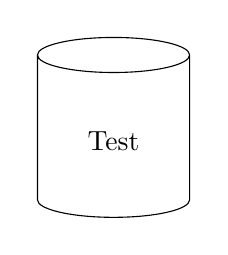
\begin{tikzpicture}
    \node (database) {\drawdatabase{Test}};
  \end{tikzpicture}
  
\begin{tikzpicture}
    \node (document) {\drawdocument{Test}};
  \end{tikzpicture}
  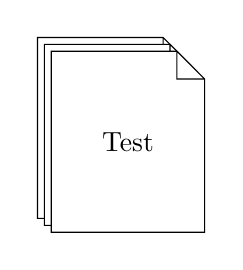
\begin{tikzpicture}
    \node (corpus) {\drawcorpus{Test}};
  \end{tikzpicture}
%%%%%%%%%%%%%%%%%%%%%%%%%%%%%%%%%%%%%%%%%%%%%%%%%%%%%%%%%%%%%%%%%%%%%%%%%%%%%%%%
  \section{Experiments}
\label{sec:experiments}
    We validate the effectiveness of our proposed candidate selection method by using two series of experiments.
    First, we provide a qualitative evaluation of the keyphrase candidates produced by our method and perform a comparison with the other methods.
    Second, we conduct an end-to-end evaluation by exploiting two keyphrase extraction systems.
    
    \subsection{Experimental settings}
    \label{subsec:experimental_settings}
        To quantify the capacity of the candidate selection methods to provide suitable candidates and avoid irrelevant ones, we compute the number of selected candidates (Cand./Doc.) and confront it with the best possible performance (maximum recall~--~R$_{\text{max}}$).
        To do so, we compute a quality ratio (QR):
        \begin{align}
            \text{QR} &= \frac{\text{R$_{\text{max}}$}}{\text{Cand./Doc.}} \times 100
        \end{align}
        The higher is QR, the better.

        \begin{table*}
            \centering
            \begin{tabular}{r|ccc|ccc|ccc}
                \toprule
                \multirow{2}{*}[-2pt]{\textbf{Method}} & \multicolumn{3}{c|}{\textbf{DUC} (\textit{English})} & \multicolumn{3}{c|}{\textbf{SemEval} (\textit{English})} & \multicolumn{3}{c}{\textbf{DEFT} (\textit{French})}\\
                \cline{2-10}
                & Cand./Doc. & R$_{\text{max}}$ & QR & Cand./Doc. & R$_{\text{max}}$ & QR & Cand./Doc. & R$_{\text{max}}$ & QR\\
                \hline
                \{1..3\}-grams & $~~~$596.2 & \textbf{90.8} & 15.2 & 2580.5 & \textbf{72.2} & $~~$2.8 & 4070.2 & \textbf{74.1} & $~~~$1.8\\
                Longest NPs & $~~~$155.6 & 88.7 & 57.0 & $~~~$646.5 & 62.4 & $~~$9.7 & $~~~$914.5 & 61.1 & $~~$6.7\\
                NP-chunks & $~~~$149.9 & 76.0 & 50.7 & $~~~$598.4 & 56.6 & $~~$9.5 & $~~~$812.3 & 63.0 & $~~$7.8\\
                LR-NPs & \textbf{$~~~$143.8} & 85.3 & \textbf{59.3} & \textbf{$~~~$538.2} & 59.4 & \textbf{11.0} & \textbf{$~~~$738.2} & 60.1 & \textbf{$~~$8.1}\\
                \bottomrule
            \end{tabular}
            \caption{Qualitative comparison of the keyphrase candidate selection methods
                     \label{tab:candidate_extraction_statistics}}
        \end{table*}

        \begin{table*}
            \centering
            \resizebox{\linewidth}{!}{
            \begin{tabular}{r@{~}|c@{~~}c@{~~}c@{~}|@{~}c@{~~}c@{~~}c@{~}|@{~}c@{~~}c@{~~}c@{~}|@{~}c@{~~}c@{~~}c@{~}|@{~}c@{~~}c@{~~}c@{~}|@{~}c@{~~}c@{~~}c}
                \toprule
                \multirow{2}{*}[-2pt]{\textbf{Method}} & \multicolumn{6}{c@{~}|@{~}}{\textbf{DUC} (\textit{English})} & \multicolumn{6}{c@{~}|@{~}}{\textbf{SemEval} (\textit{English})} & \multicolumn{6}{c}{\textbf{DEFT} (\textit{French})}\\
                \cline{2-19}
                & \multicolumn{3}{c@{~}|@{~}}{TF-IDF} & \multicolumn{3}{c@{~}|@{~}}{KEA} & \multicolumn{3}{c@{~}|@{~}}{TF-IDF} & \multicolumn{3}{c@{~}|@{~}}{KEA} & \multicolumn{3}{c@{~}|@{~}}{TF-IDF} & \multicolumn{3}{c}{KEA}\\
                \cline{2-19}
                & P & R & F & P & R & F & P & R & F & P & R & F & P & R & F & P & R & F\\
                \hline
                \{1..3\}-grams & 14.3 & 19.0 & 16.1$~~$ & 12.0 & 16.6 & 13.7$~~$ & $~~$9.0 & $~~$6.6 & $~~$7.2$~~$ & 19.4 & 13.7 & 15.9 & $~~$6.7 & 12.5 & $~~$8.6 & 13.4 & 25.3 & 17.3\\
                Longest NPs & 24.2 & 31.7 & 27.0$~~$ & \textbf{14.5} & 19.9 & 16.5$~~$ & 11.7 & $~~$7.9 & $~~$9.3$~~$ & 19.6 & 13.7 & 16.0 & $~~$9.5 & 17.6 & 12.1 & 14.1 & 26.3  &18.1\\
                NP-chunks & 21.1 & 28.1 & 23.8$~~$ & 13.5 & 18.6 & 15.4$~~$ & 11.9 & $~~$8.0 & $~~$9.5$~~$ & 19.5 & 13.7 & 16.0 & $~~$9.6 & 17.9 & 12.3 & 14.3 & 26.8 & 18.4\\
                LR-NPs & \textbf{24.3} & \textbf{32.0} & \textbf{27.2$^\dagger$} & \textbf{14.5} & \textbf{20.0} & \textbf{16.6$^\ddagger$} & \textbf{12.4} & \textbf{$~~$8.4} & \textbf{$~~$9.9$^\ddagger$} & \textbf{20.4} & \textbf{14.4} & \textbf{16.7}& \textbf{10.1} & \textbf{18.5} & \textbf{12.9} & \textbf{14.4} & \textbf{27.0} & \textbf{18.6}\\
                \bottomrule
            \end{tabular}
            }
            \caption{Comparison of TF-IDF and KEA applied on top of different candidate selection methods.
            $\ddagger$ indicates a significant improvement overall candidate sets and $\dagger$ indicates a significant improvement overall candidate sets but the longest NPs at 0.001 level using Student's t-test.
                     \label{tab:keyphrase_extraction_results}}
        \end{table*}
        
        We measure the impact of each candidate selection method on the keyphrase extraction task using the two following unsupervised and supervised keyphrase extraction methods:
        \begin{itemize}
            \item{\textbf{TF-IDF~\cite{jones1972tfidf}:} Word significancy weighting scheme.
                  Words are weighted based on their frequency in the document and the inverse number of documents in which they appear (specificity);
                  Candidates are weighted using the sum of  their words' score.}
            \item{\textbf{KEA~\cite{witten1999kea}:} Naive Bayes classifier trained on two features: the TF-IDF\footnote{KEA computes a TF-IDF based on candidate frequency, whereas our TF-IDF baseline relies on word frequency. KEA's TF-IDF is more efficient on larger documents than smaller ones.} and the first position of each candidate selected within train documents.}
        \end{itemize}
        We report the performance of TF-IDF and KEA in terms of precision~(P), 
        recall~(R) and F1-measure (F) at the top 10 keyphrases.
        Candidate and reference keyphrases are stemmed to reduce the number 
        of mismatches.
    
    \subsection{Candidate selection evaluation}
    \label{subsec:candidate_extraction_evaluation}
        Table~\ref{tab:candidate_extraction_statistics} presents the results of the intrinsic evaluation of the candidate selection methods.
        %Unsurprisingly, the best maximum recall is achieved by the $\{1..3\}$-grams selection method, but at the cost of a huge number of unrelevant candidates as indicated by the low quality ratio.
        Unsurprisingly, the best maximum recall is achieved when selecting $\{1..3\}$-grams, but at the cost of a huge number of irrelevant candidates as indicated by the low QR.
        Among the other selection methods, our method shows a competitive maximum recall while reducing the number of candidates.
        As a consequence, the LR-NPs quality outperforms other selected candidates quality, which is crucial as it directly affects the performance and time complexity of keyphrase extraction methods~\cite{wang2014keyphraseextractionpreprocessing}.
        
        \TODO{examples of true and false positives}
    
    \subsection{Keyphrase extraction evaluation}
    \label{subsec:keyphrase_extraction_evaluation}
        Table~\ref{tab:keyphrase_extraction_results} shows the results of the extrinsic evaluation of the candidate selection methods.
        Overall, we observe that the performance of TF-IDF and KEA is closely correlated with the quality of the set of selected candidates.
        Best results are then obtained when TF-IDF and KEA are applied on LR-NPs (half of them are significantly better).
        Thus, although our proposed selection method does not achieve the best maximum recall, it still outperforms the other candidate selection  methods.
        Comparing longest NPs, NP-chunks and LR-NPs demonstrates that it is efficient to use heuristic based on linguistic properties.

  \section{Conclusion et perspectives}
\label{sec:conclusion_et_perspectives}
  Dans cet article, nous nous intéressons à la tâche d'extraction automatique de
  termes-clés dans les documents scientifiques et émettons l'hypothèse que sa
  difficulté est variable selon la discipline des documents traités. Pour
  vérifier cette hypothèse, nous disposons de notices bibliographiques réparties
  dans cinq disciplines (archéologie, linguistique, sciences de l'information,
  psychologie et chimie) auxquelles nous appliquons six systèmes d'extractions
  automatique de termes-clés différents. En comparant les termes-clés extraits
  par chaque système avec les termes-clés de référence assignés aux notices dans
  des conditions réels d'indexation, notre hypothèse se vérifie et nous
  observons l'échelle suivante (de la discipline la plus facile à la plus
  difficile)~:
  \begin{enumerate*}
    \item{Archéologie~;}
    \item{Linguistique~;}
    \item{Sciences de l'information~;}
    \item{Psychologie~;}
    \item{Chimie.}
  \end{enumerate*}

  À l'issue de nos expériences et de nos observations du contenu des notices,
  nous constatons deux facteurs ayant un impact sur la difficulté de la tâche
  d'extraction automatique de termes-clés. Tout d'abord, nous observons que
  l'organisation du résumé peut aider l'extraction de termes-clés. Un résumé
  riche en explications et en mises en relations des différents concepts est
  moins difficile à traiter qu'un résumé énumératif pauvre en explications.
  Ensuite, le vocabulaire utilisé dans une discipline peut influer sur la
  difficulté à extraire les termes-clés des documents de cette discipline. Si le
  vocabulaire spécifique contient des composés syntagmatiques dont certains
  éléments sont courants dans la discipline, alors il peut être plus difficile
  d'extraire les termes-clés des documents de cette discipline.

  Des deux facteurs identifiés émergent plusieurs perspectives de travaux
  futurs. Il peut être intéressant d'analyser le discours des documents afin de
  mesurer, en amont, le degré de difficulté de l'extraction de termes-clés. Avec
  une telle connaissance, nous pourrions proposer une méthode capable de
  s'adapter au degré de difficulté en ajustant automatiquement son paramètrage.
  Cependant, l'analyse que nous proposons dans cet article se fonde uniquement
  sur le contenu de notices appartenant à cinq disciplines. Il serait pertinent
  d'étendre cette analyse au contenu intégral des documents scientifiques, ainsi
  que d'élargir le panel de disciplines utilisées dans ce travail, afin
  d'établir des catégories de discplines plus ou moins difficiles à traiter
  (p.~ex. la chimie fait partie des disciplines expérimentales, qui sont
  difficiles à traiter). Nous oberservons aussi que le vocabulaire utilisé dans
  une discipline, en particulier celui utilisé pour les termes-clés, peut rendre
  la tâche d'extraction automatique de termes-clés plus difficile. Il est donc
  important de bénéficier de resources telles que des thésaurus pour permettre à
  une méthode d'extraction de termes-clés de s'adapter au domaine. Pour
  TopicRank, par exemple, avoir connaissance de la terminologie utilisée dans
  une discipline peut améliorer le choix du terme-clé le plus représentatif d'un
  sujet. Enfin, il serait intéressant de penser la tâche d'extraction de
  termes-clés comme une tâche d'extraction d'information pour le remplissage
  d'un formulaire. En archéologie, par exemple, il pourrait s'agir d'extraire
  les informations géographiques (pays, régions, etc.), chronologiques (période,
  culture, etc.), ou encore environnementales (animaux, végétaux, etc.).



%  \section*{Acknowledgements}
%  The authors would like to thank the anonymous reviewers for their useful
%  advice and comments. This work was supported by the French National Research
%  Agency (TermITH project -- ANR-12-CORD-0029).

  % include your own bib file like this:
  \bibliographystyle{acl}
  \bibliography{../../biblio}
\end{document}
